\section{Task 3: The robot's kinematic diagram}
\FloatBarrier % Now figures cannot float above section title

As we can see in the \autoref{F 4.1}, we can find that all the z-axis are the revolution or direction of every joints, and use the right-hand rule, we can check if all the x-axis are perpendicular both to its own z axis and the z axis of the frame before it. Apparently, the directions of all the axis are strictly following the Devenit-Hartenburg Framerules.

\begin{figure}[htbp]
    \centering
    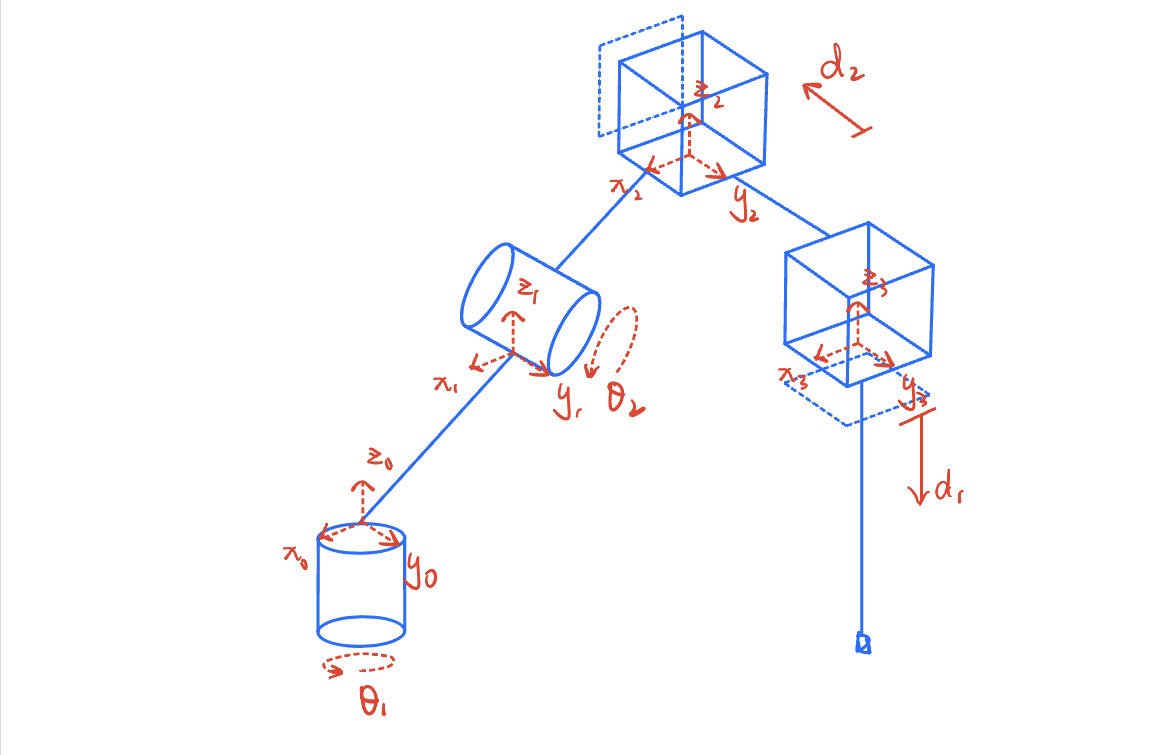
\includegraphics[width=7cm]{./fig/D-H.jpg}
    \caption{The robot's kinematic diagram}
    \label{F 4.1}
\end{figure}
